\documentclass[german]{latteachCD}
\usepackage{mdframed}
\usepackage{amsmath}
\usepackage{amsfonts}
\usepackage{amssymb}
%\usepackage{wasysym}
%\usepackage{stmaryrd}
%\usepackage{fixltx2e}
%\usepackage{enumitem}
\usepackage{extarrows}
\newcommand{\abs}[1]{\lvert#1\rvert}

\usepackage{tikz}
\usetikzlibrary{arrows,automata,positioning,shapes,calc,decorations.pathmorphing,matrix}

\tikzstyle{automaton}=[->, >=stealth', initial text=, auto, node distance=20mm, bend angle=20, semithick, x=20mm, y=20mm]
\tikzset{
  every state/.style={
    inner sep=0pt,
    minimum size=8mm
  },
  small state/.style={
      state,
      minimum size=3mm
  },
  ellipse state/.style={
    draw,
    shape=ellipse,
    minimum width=20mm,
    minimum height=12.36mm,
    text width=14.5mm,
    inner sep=0mm,
    path picture={
      \draw (path picture bounding box.east) ellipse [x radius=9mm, y radius=9mm];
    }
  },
  accepting ellipse state/.style={
    ellipse state,
    path picture={
      \clip (path picture bounding box.east) ellipse [x radius=9.4mm, y radius=9.4mm];
      \draw[double] (path picture bounding box.east) ellipse [x radius=9mm, y radius=9mm];
      \draw[double] (path picture bounding box.center) ellipse [x radius=10mm, y radius=6.18mm];
    }
  }
}

  
%%%%%%%%%%%%%%%%%%%%%%%%%%%%%%%%%%%%%%%%%%%%%%%%%%%%%%%%%%%%%%%%%%%%%%%%%%%%%%%%%%%%%%%%%%%%

\usepackage{xspace}

\author{~}
\term{Wintersemester 2017/18}
\title{\Large 3.\@ Übungsblatt}
\course{\LARGE Formale Systeme}

\usepackage{csquotes}
\usepackage{booktabs}
\usepackage{amsmath}
\usepackage{amsfonts}
\usepackage{amssymb}
\usepackage{mathtools}
\usepackage{wasysym}
\usepackage{stmaryrd}
\usepackage{enumitem}
\usepackage{tikz}
\usepackage{makecmds}

\renewcommand{\epsilon}{\varepsilon}
\renewcommand{\phi}{\varphi}
\renewcommand{\rho}{\varrho}
\renewcommand{\theta}{\vartheta}
\newcommand{\tuple}[1]{\langle{#1}\rangle} 

\newcommand{\size}[1]{\ensuremath{\lvert #1\rvert}}
\newcommand{\gdw}{\mathrel{\mathrm{gdw.}}}
\newcommand{\falls}{\mathrel{\mathrm{falls}}}

\provideenvironment{solution}{\textbf{Lösung}:}{}
\usepackage{comment}

\usepackage{etex,etoolbox}

\DeclareRobustCommand{\NN}{\ensuremath{\mathbb{N}}}

\newbool{Baader}
\newbool{Kroetzsch}
\booltrue{Kroetzsch}

\DeclareMathOperator{\Var}{Var}
\ifbool{Baader}{%
  \DeclareMathOperator{\Unt}{Unt}
  \DeclareMathOperator{\Res}{Res}
}{}
\ifbool{Kroetzsch}{%
  \DeclareMathOperator{\Unt}{Sub}
  \DeclareMathOperator{\Res}{Res}
  \usepackage{multicol}         % for resolution
}{}

\excludecomment{solution}

\begin{document}

\maketitle

\begin{center}
\begin{mdframed}
  \renewcommand{\theexercise}{zur Selbstkontrolle
  (diese werden in den Übungen nicht besprochen)}
  
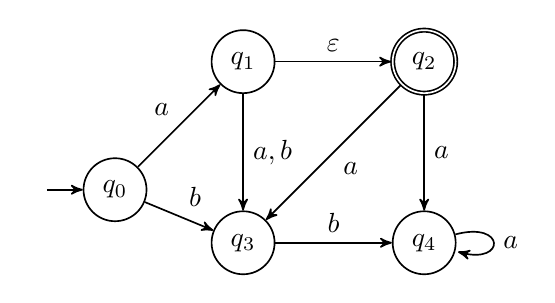
\begin{tikzpicture} [->, >=stealth', initial text=, auto, node
  distance=23mm, bend angle=20, semithick]%[node distance=2cm,auto]
 \node[state,initial] (q_0) {$q_0$}; 
 \node[state] (q_1) [above right of=q_0] {$q_1$}; 
 \node[state,accepting] (q_2) [right of=q_1] {$q_2$}; 
 \node[state] (q_3) [below of=q_1] {$q_3$};
 \node[state] (q_4) [right of=q_3] {$q_4$};
 \path[->]
  (q_0) edge node {$a$} (q_1) 
  (q_0) edge node {$b$} (q_3) 
  (q_1) edge node {$a, b$} (q_3) 
  (q_1) edge node {$\varepsilon$} (q_2) 
  (q_2) edge node {$a$} (q_3) 
  (q_2) edge node {$a$} (q_4) 
  (q_3) edge node {$b$} (q_4)
  (q_4) edge [loop right] node {$a$} (q_4) ;
\end{tikzpicture}

%  {\bfseries Hinweis:} Die Aufgaben *) und **) 
%  dienen der Selbstkontrolle und werden in der
%  Übung nicht besprochen.  
\end{mdframed}
\end{center}

\setcounter{exercise}{0}


\begin{exercise}

Zeigen Sie konstruktiv, dass 
\begin{itemize}
 \item für jeden NFA $\mathcal{M}$ mit mehreren Startzuständen ein äquivalenter NFA $\mathcal{M'}$ mit nur einem Startzustand existiert bzw. 
 \item für jeden NFA $\mathcal{M}$ mit mehreren Finalzuständen ein äquivalenter NFA $\mathcal{M'}$ mit nur einem Finalzustand existiert. Gilt die letzte Aussage auch für DFAs?
\end{itemize}
\end{exercise}

	

\newpage
\begin{exercise}

Bearbeiten Sie eine der vier folgenden Fragestellungen:

\begin{enumerate}
\item [(a)]
Seien $L$, $K$  regul\"are Sprachen \"uber einem Alphabet $\Sigma$.
Zeigen Sie, da{\ss}
$$L/K \ = \ \{ x \in \Sigma^* : xy \in L \ \mbox{f\"ur ein
$y \in K$} \}$$ 
regul\"ar ist.

\item [(b)]
Sei $L$ eine regul\"are Sprache \"uber einem mindestens
zweielementigen Alphabet $\Sigma$.
Zeigen Sie, da{\ss} die folgende Sprache regul\"ar ist.

$L_1 =  \{ x \in L : \mbox{es gibt kein $y \in \Sigma^+$,
so da{\ss} $xy \in L$} \}$

\item [(c)]
Sei $L$ eine regul\"are Sprache \"uber einem mindestens
zweielementigen Alphabet $\Sigma$.
Zeigen Sie, da{\ss} die folgende Sprache regul\"ar ist.

$L_2 = \{ x \in L : \mbox{kein echtes Pr\"afix von $x$ liegt in $L$}
\}$

\item [(d)] Sei $L$ eine regul\"are Sprache \"uber einem mindestens
zweielementigen Alphabet $\Sigma$. Zeigen Sie, da{\ss} die Spiegelbildsprache 
$L^R = \{a_n a_{n-1} \ldots a_0 \in\Sigma^* \mid a_0 \ldots a_{n-1} a_n \in L\}$ 
wiederum eine reguläre Sprache ist. 

\end{enumerate}
\end{exercise}


\begin{exercise}

Es sei $L$ die Sprache aller $w \in \{ 0, 1 \}^{ + } $ mit
  gleich vielen Nullen wie Einsen. Man gebe f"ur diese Sprache eine
  kontextfreie Grammatik an.
  Beweisen Sie die Korrektheit und Vollst\"andigkeit Ihrer L\"osung!
\end{exercise}


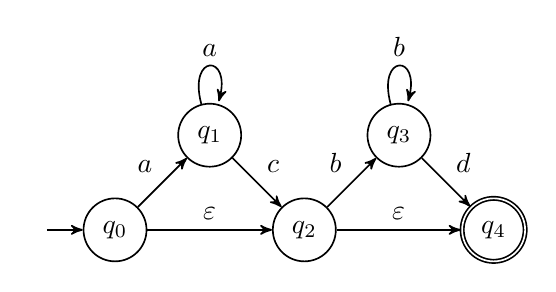
\begin{tikzpicture} [->, >=stealth', initial text=, auto, node
  distance=17mm, bend angle=20, semithick]
   \node[state,initial,initial text= ] (q0) {$q_0$};
   \node[state] (q1) [above right of=q0] {$q_1$};
   \node[state] (q2) [below right of=q1] {$q_2$};
   \node[state] (q3) [above right of=q2] {$q_3$};
   \node[state,accepting] (q4) [below right of=q3] {$q_4$};

   \path[->] (q0) edge               node {$a$} (q1) 
                  edge               node {$\varepsilon$} (q2) 
             (q1) edge  [loop above] node {$a$} (q1) 
                  edge               node {$c$} (q2) 
             (q2) edge               node {$b$} (q3) 
                  edge               node {$\varepsilon$} (q4) 
             (q3) edge  [loop above] node {$b$} (q3) 
                  edge               node {$d$} (q4) ;
\end{tikzpicture}
\newpage
\begin{exercise}
  Gegeben sind die Automaten
  \begin{align*}
     \mathcal{M}_1 &=(\{q_0,\dots,q_3\},\{a,b\},\delta_1,\{q_0\},\{q_2,q_3\}),
    &\mathcal{M}_2 &=(\{p_0,\dots,p_3\},\{a,b\},\delta_2,\{p_0\},\{p_3\}),\\
     \mathcal{M}_3 &=(\{s_0,\dots,s_3\},\{a,b\},\delta_3,\{s_0\},\{s_3\})\ \text{und}
    &\mathcal{M}_4 &=(\{t_0,\dots,t_5\},\{a,b\},\delta_4,\{t_0\},\{t_3,t_5\})
  \end{align*}
  mit

  \begin{center}
    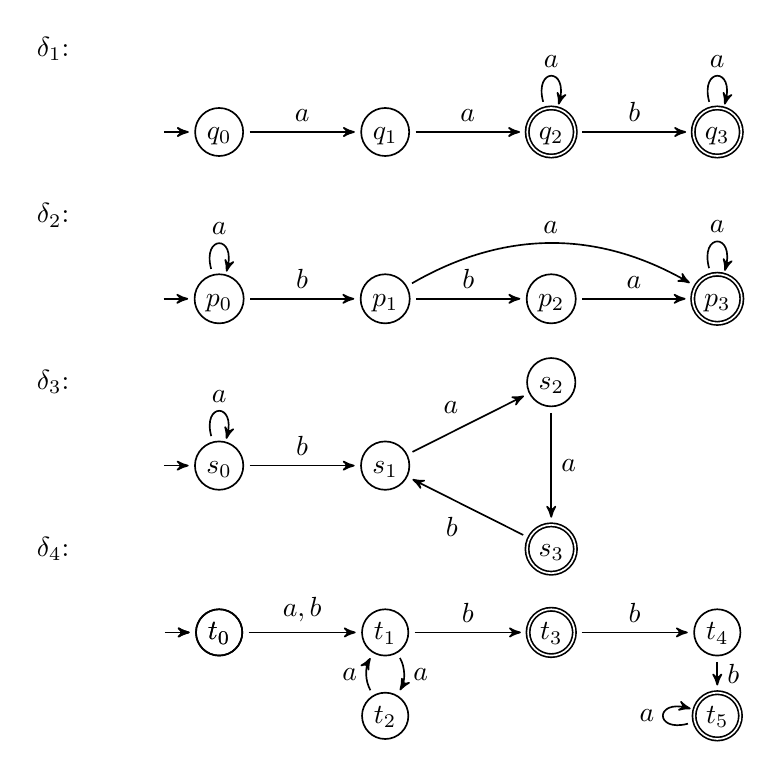
\begin{tikzpicture}[%
        ->,
        >=stealth',
        semithick,
        initial text=,
        shorten <=2pt,
        shorten >=2pt,
        auto,
        on grid,
        node distance=7ex and 6em,
        every state/.style={minimum size=0pt,inner sep=2pt,text height=1.5ex,text depth=.25ex},
        bend angle=30]
      \node                  (delta_1)                          {$\delta_1$:};
      \node[state,initial]   (q_0)     [below right=of delta_1] {$q_0$};
      \node[state]           (q_1)     [right=of q_0]           {$q_1$};
      \node[state,accepting] (q_2)     [right=of q_1]           {$q_2$};
      \node[state,accepting] (q_3)     [right=of q_2]           {$q_3$};
      \path[->] (q_0) edge              node {$a$}   (q_1)
                (q_1) edge              node {$a$}   (q_2)
                (q_2) edge [loop above] node {$a$}   (q_2)
                      edge              node {$b$}   (q_3)
                (q_3) edge [loop above] node {$a$}   (q_3);
      \node                  (delta_2) [below left=of q_0]      {$\delta_2$:};
      \node[initial,state]   (p_0)     [below right=of delta_2] {$p_0$};
      \node[state]           (p_1)     [right=of p_0]           {$p_1$};
      \node[state]           (p_2)     [right=of p_1]           {$p_2$};
      \node[state,accepting] (p_3)     [right=of p_2]           {$p_3$};
      \path[->] (p_0) edge [loop above]  node {$a$} (p_0)
                (p_0) edge               node {$b$} (p_1)
                (p_1) edge               node {$b$} (p_2)
                (p_1) edge [bend left]   node {$a$} (p_3)
                (p_2) edge               node {$a$} (p_3)
                (p_3) edge [loop above]  node {$a$} (p_3);
      \node                  (delta_3) [below left=of p_0]      {$\delta_3$:};
      \node[state,initial]   (s_0)     [below right=of delta_3] {$s_0$};
      \node[state]           (s_1)     [right=of s_0]           {$s_1$};
      \node[state]           (s_2)     [above right=of s_1]     {$s_2$};
      \node[state,accepting] (s_3)     [below right=of s_1]     {$s_3$};
      \path[->] (s_0) edge [loop above] node {$a$}   (s_0)
                (s_0) edge              node {$b$}   (s_1)
                (s_1) edge              node {$a$}   (s_2)
                (s_2) edge              node {$a$}   (s_3)
                (s_3) edge              node {$b$}   (s_1);
      \node                  (delta_4) [below left=of s_0]      {$\delta_4$:};
      \node[initial,state]   (t_0)     [below right=of delta_4] {$t_0$};
      \node[initial,state]   (t_0)     [below right=of delta_4] {$t_0$};
      \node[state]           (t_1)     [right=of t_0]           {$t_1$};
      \node[state]           (t_2)     [below=of t_1]           {$t_2$};
      \node[state,accepting] (t_3)     [right=of t_1]           {$t_3$};
      \node[state]           (t_4)     [right=of t_3]           {$t_4$};
      \node[state,accepting] (t_5)     [below=of t_4]           {$t_5$};
      \path[->] (t_0) edge              node {$a,b$} (t_1)
                (t_1) edge [bend left]  node {$a$}   (t_2)
                (t_1) edge              node {$b$}   (t_3)
                (t_2) edge [bend left]  node {$a$}   (t_1)
                (t_3) edge              node {$b$}   (t_4)
                (t_4) edge              node {$b$}   (t_5)
                (t_5) edge [loop left]  node {$a$}   (t_5);
    \end{tikzpicture}   
  \end{center}

  \vspace*{2ex}

  \begin{enumerate}
    \item Konstruieren Sie einen $\varepsilon$-freien NFA~$\mathcal{M}_a$ mit
      $L(\mathcal{M}_a)=L(\mathcal{M}_1)\cap L(\mathcal{M}_2)$.
      Dabei dürfen Sie sich auf die vom Startzustand erreichbaren Zustände
      beschränken.
    \item Konstruieren Sie einen $\varepsilon$-freien NFA~$\mathcal{M}_b$ mit
      $L(\mathcal{M}_b)=L(\mathcal{M}_1)^*$.
    \item Konstruieren Sie einen $\varepsilon$-freien NFA~$\mathcal{M}_c$ mit
      $L(\mathcal{M}_c)=L(\mathcal{M}_3)\cup L(\mathcal{M}_4)$.
    \item Konstruieren Sie einen $\varepsilon$-freien NFA~$\mathcal{M}_d$ mit
      $L(\mathcal{M}_d)=L(\mathcal{M}_3)\circ L(\mathcal{M}_4)$.
  \end{enumerate}
\end{exercise}




% hätten auch noch gepasst:
%\newpage
%\input{pool/baier/52}
%\input{pool/baier/55}
%\input{pool/baier/61}
%\input{pool/baier/692}
%\input{pool/baier/71}
%\input{pool/baier/712}
%\input{pool/baier/723}
%\input{pool/baier/726}
%\input{pool/baier/742}
%\input{pool/baier/k2_2a}

\end{document}
